%Einleitung zur Implementierung
%Sprache, Stiel, Debugging, IDE, etc.
\section{Entwicklungsumgebung}
Zur Entwicklung der Softwarekomponente soll erst Keil\textsuperscript{\scriptsize\textregistered} Microcontroller Development Kit (MDK) auf einem Rechner installiert werden. Das Kit ist besonders gut geeignet für Arm\textsuperscript{\scriptsize\textregistered}-basierte Microcontroller und beinhaltet alle notwendigen Komponente für Embedded Applikationen. Die Edition MDK-Lite ist konstenlos jedoch mit der Beschränkung von 32KBytes Codegröße verfügbar. Zusätzlich muss Legacy Package ARMv7 (NXP LPC 2388) installiert werden. Anschließend soll die Integrierte Entwicklungsumgebung Keil $\mu$version 5 erfolgreich installiert sein.

Der Board kann durch einen USB-Anschluss vom Rechner eingeschaltet werden. Der ULINK-ME kann ebenfalls durch einen USB-Anschluss zum Laden des Programms und zum Debuggen verwendet werden.
Die Software für den RaspberryPi 1B wurde mit den \texttt{arm-none-eabi gcc}, basierend auf \texttt{GCC 4.5.2} von CodeSourcery kompilliert.

Sämtlicher Quellcode des Projekts wurde in C geschrieben und Doxygen-konform dokumentiert.

%Beschreibung der Konfiguration von IDE

\section{Pinbelegung}

\begin{figure}
	\centering
	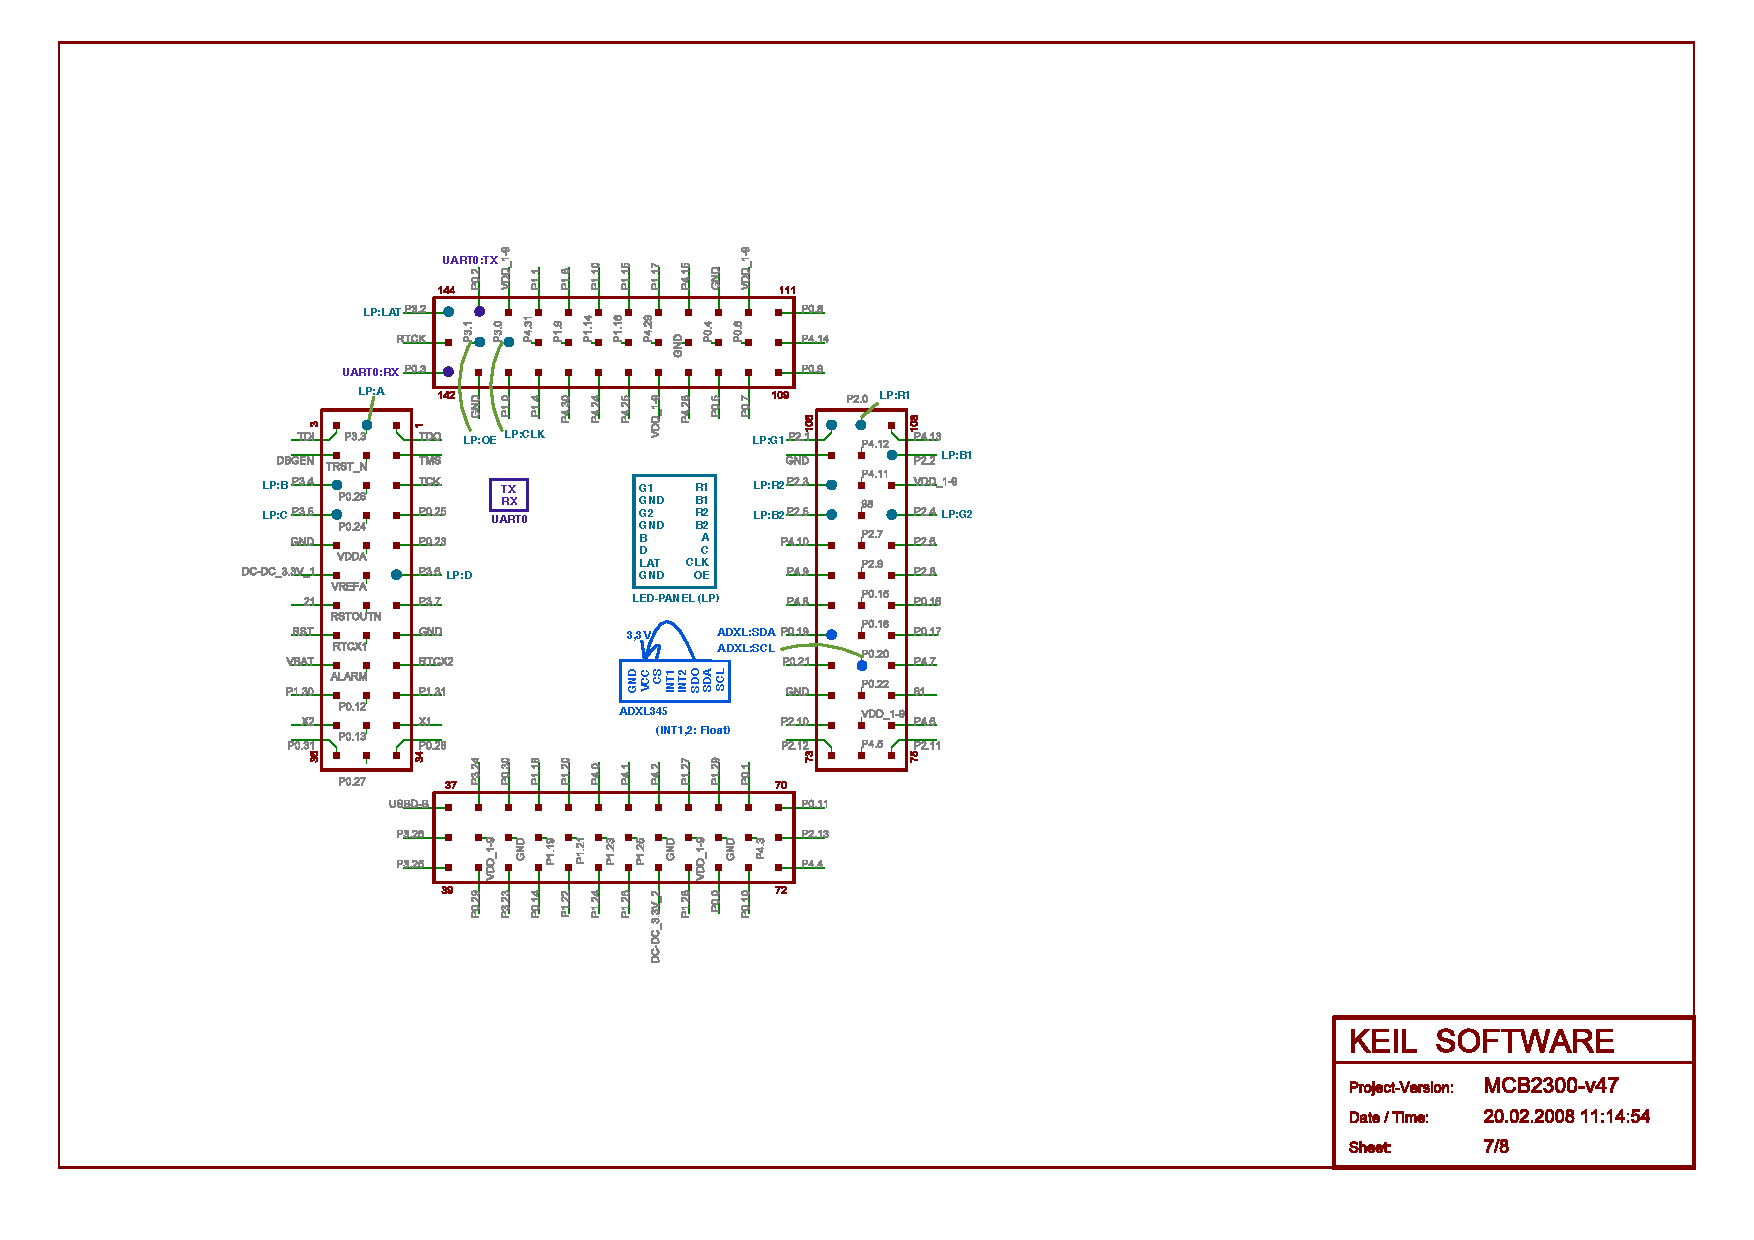
\includegraphics[clip, trim=4cm 5cm 13cm 5cm, width=.99\textwidth]{pinbelegung}
	\caption[Pinbelegung]{Pinbelegung}
	\label{fig:pins}
\end{figure}

Der Beschleunigungssensor und eines der 6 Panele werden durch freie GPIO-Pins mit dem Board verbunden. Abbildung \ref{fig:pins} zeigt die genutzte Pinbelegung. Es ist dabei zu beachten, die bereits vom Hersteller belegten Pins des Boards zu vermeiden, andernfalls kann es zu Problemen beim Betrieb kommen. Ebenso wird ein Raspberry Pi 1B (siehe \ref{chap:impl:sph:rp}) über den \texttt{UART0} angebunden.
